\documentclass[11pt,a4paper]{article}

\usepackage[T1]{fontenc}
\usepackage[utf8]{inputenc}
\usepackage[margin=2.6cm]{geometry}
\usepackage{graphicx}
\usepackage{booktabs}
\usepackage{amsmath}
\usepackage{microtype}
\usepackage[hidelinks]{hyperref}
\usepackage[numbers,sort&compress]{natbib}
\usepackage{caption}
\captionsetup{font=small,labelfont=bf}
\usepackage{parskip}

\title{\textbf{Lunar Metropolis}: an agent-driven simulation of lunar city
growth, and what it says about the balance between surface settlement and
subsurface arcologies}

\author{Richard Barker\thanks{%
  \textbf{TODO before deposit:} affiliation. \\
  \textbf{TODO before deposit:} ORCID. \\
  Correspondence via the repository:
  \url{https://github.com/dr-richard-barker/LunarSims}}}

\date{\today}

\begin{document}
\maketitle

\begin{abstract}
\noindent
We describe \emph{Lunar Metropolis}, an executable model of lunar settlement
growth built as a playable simulation, and report what the model says about
where people can be housed on the Moon. The model couples an elevation field
to a solar-exposure raycast, and from that single coupling derives both the
distribution of water ice and the economic value of ground. Three habitat
strategies are represented: surface construction, arcologies bored downward
into permanently shadowed ice deposits, and arcologies extending along
pre-existing lava tubes. We calibrate the model's resource parameters against
its own generated worlds, verify its behaviour with a suite of 130 scenarios
performing 12{,}322 simulated days across 265 generated worlds per pass, and
compare the three strategies on a common footing. The central result is that
subsurface habitation in this model does not save money --- it costs between
17 and 76 times more per resident than surface construction --- but buys
surface area, at up to 2{,}295 residents per occupied surface tile against 62
for the best surface alternative. A second result is that the three strategies
are not equally available: at realistic latitudes, subsurface habitation is
effectively a polar privilege, with equatorial mare sites offering a median of
2 ice tiles and no lava tubes at all. We describe the model, its calibration,
its verification methodology, and four classes of failure that were detectable
only by running it. Everything reported is regenerable from the accompanying
software.
\end{abstract}

\section{Introduction}

Most models of lunar settlement are written to answer a question that has
already been posed. A structural analysis asks whether a given span will
stand \citep{blair2017stability}; a thermal model asks what a given shell
costs to keep warm. Such models are precise about a narrow thing.

This work takes the opposite approach. \emph{Lunar Metropolis} is an
executable model of a settlement as a whole --- terrain, illumination,
volatiles, three utility networks, an economy, and a population that responds
to all of them --- built as a playable simulation and then interrogated as a
model. It is deliberately imprecise about every individual mechanism, and in
exchange it can be run end to end, tens of thousands of simulated days at a
time, across hundreds of independently generated worlds. What such a model is
good for is not predicting a number but exposing a \emph{structure}: which
constraints bind, which trade against which, and which supposedly free choices
turn out to have been made by the terrain generator before the player arrived.

The specific question we put to it here is the balance between building on the
lunar surface and building underneath it. The case for going underground is
well rehearsed. Burial under regolith reduces the galactic cosmic ray dose,
though not as simply as one might expect: secondary neutrons, pions and photons
produced within the shield itself first \emph{rise} with shell thickness before
falling away \citep{jia2010radiation}. An intact lava tube offers a large
shielded volume that nobody has to excavate, and the protection is substantial
--- a Monte Carlo study puts the effective dose equivalent inside a horizontal
lunar tube below $1$~mSv\,yr$^{-1}$, against $416$~mSv\,yr$^{-1}$ on the open
surface \citep{naito2020radiation} --- in voids whose morphology at Marius Hills
was mapped from imagery decades ago \citep{greeley1971mariushills} and whose
presence there is supported by radar sounding \citep{kaku2017intact}. What is less often stated is
what the choice \emph{costs}, in a currency that lets it be compared against
simply building on the surface instead. That is the question this model is
shaped to answer.

Two features of the Moon do most of the work in the model, and both are
consequences of illumination. Near the poles the Sun tracks close to the
horizon, so modest relief casts enormous shadows, and crater floors that never
see the Sun act as cold traps where water ice is stable
\citep{paige2010diviner}; the LCROSS impact into Cabeus returned direct
evidence of water in such a deposit \citep{colaprete2010water}. The same
illumination geometry that puts the ice there also makes that ground worthless
to build on: it is dark, cold, and generates no solar power. The model derives
both facts from one raycast, and the tension between them is the engine of
everything reported below.

We make three contributions. First, we describe the model and the reasoning
behind its structure (Sections~\ref{sec:model}--\ref{sec:habitats}). Second, we
calibrate its resource parameters against its own generated worlds rather than
by hand, and report the calibration
(Section~\ref{sec:calibration}). Third, we report what the model says about the
surface/subsurface balance, and what it says about the automated director that
plays it (Sections~\ref{sec:results}--\ref{sec:failures}). We are explicit
throughout about which statements are results of the model and which are
assumptions built into it; Section~\ref{sec:limitations} is devoted to the
difference.

\section{The model}
\label{sec:model}

\subsection{Scale and structure}

The model is a discrete simulation on a $128\times128$ grid of $16{,}384$
tiles, each carrying an integer elevation on 16 levels, a terrain type, a solar
exposure, a dust loading, and optionally a mineral deposit. One tick is one
simulated day. The implementation is approximately $12{,}800$ lines of
dependency-free JavaScript across 20 modules, governed by 52 named constants
collected in a single table so that every tunable quantity is visible in one
place.

The choice of a coarse integer grid over a continuous field is deliberate. The
model's purpose is to expose which constraints bind against each other, and
that structure survives discretisation; what discretisation buys is the ability
to run a complete settlement history in a few seconds, which is what makes the
sweeps in Section~\ref{sec:results} affordable.

\subsection{Illumination, and what follows from it}

Elevation is the primary field; everything else is derived. Each tile's solar
exposure is computed by casting rays outward in eight directions and testing
whether the local horizon occludes the Sun, with the horizon rise per unit
distance --- the parameter \texttt{sunSlope} --- set from the site's latitude.
Near the pole this parameter is small, so even shallow relief occludes, and
deep crater floors receive an exposure of exactly zero.

From that one field the model derives, in order:

\begin{itemize}
\item \textbf{Where ice is.} Ice is placed only where exposure falls below a
  shadow threshold, with richness increasing as exposure falls further. This
  reproduces the qualitative structure of polar cold traps
  \citep{paige2010diviner} without attempting their actual distribution.
\item \textbf{What power is available.} Photovoltaic output scales directly
  with local exposure, so the ground that holds ice generates nothing.
\item \textbf{What ground is worth.} Land value rises with exposure and with
  elevation, so shadowed floors are also the least valuable ground to build
  on.
\end{itemize}

This triple coupling is the model's central design decision. Because all three
follow from a single raycast, the antagonism between them is structural rather
than imposed: the most valuable resource sits on the least valuable ground, and
is hardest to power. No parameter tunes this relationship, and none can switch
it off.

\subsection{Networks, demand and progression}

Three utility networks must independently reach ground before it develops:
surface transit tubes, which serve by adjacency; power conduits, which
propagate a flood fill from generators and also conduct through developed
buildings; and buried atmosphere mains, which coexist with whatever occupies
the surface. Population and employment are driven by a three-index demand
model in which habitation grows while jobs outrun residents, and commerce and
industry grow while residents outrun jobs, with the two employment ratios
summing to unity so the system has a fixed point rather than a ceiling.

Colonies advance through four eras gated jointly on peak population and
accumulated research. The gate is conjunctive on purpose: population alone
would make research optional, and research alone would let a tiny well-funded
outpost build a skyline.

\section{Three ways to house a colony}
\label{sec:habitats}

The model represents three habitat strategies. They differ in where the
volume comes from, and it is that difference --- rather than any difference in
comfort or technology --- that the model is built to price.

\subsection{Surface construction}

Ground is zoned and the settlement raises buildings on it as demand and land
value allow, to a density ceiling set by the current era. A high-density
habitation tile at its final stage houses 62 residents. Surface construction
is available essentially everywhere: across all site classes tested, around
$16{,}100$ of the $16{,}384$ tiles are buildable. It is constrained not by
where it may go but by land value, by the era, and by the fact that every
zoned tile must be within one tile of all three networks.

\subsection{Bored arcologies}

Four structures excavate downward into permanently shadowed ice. They may only
be sited on an ice deposit, which --- because of the coupling described in
Section~\ref{sec:model} --- confines them to shadowed crater floors, and they
require a level pad of $3\times3$ or $5\times5$ tiles.

Each opens as a single gallery and sinks one level at a time, but only while
all three networks reach it and the colony is neither short of generating
capacity nor of pressurisation. This is the same condition under which zoned
ground develops, applied to a structure. A bore that loses its utilities stops
where it is and keeps what it has already opened.

Their yield depends on the ice within reach, summed over a radius of three
tiles and \emph{shared} with any other bore whose radius overlaps. Two bores
placed close together therefore make each other worse, which makes the
distribution of the deposit --- not merely the presence of one tile of it ---
the object of the siting decision.

The four differ in what they return. One is a pure housing structure; one
melts its ice and returns a large part of its own pressurisation; one refines
and exports, employing more people than it houses and venting dust that
degrades the ground downwind; and one, gated behind the final era, is the
largest structure in the model.

\subsection{Lava tube arcologies}

The third strategy takes a void that already exists. Where the terrain
generator carves a sinuous rille, the model records the intact tube continuing
beneath it: a course of tiles, a width, and a roof depth. A tube arcology is
sunk onto that course and then extends \emph{along} it, one tile at a time,
under the same utility condition as a bore.

Three properties distinguish it, and together they are the reason it is
modelled as its own family rather than as a fifth bore:

\begin{enumerate}
\item \textbf{The volume is free.} Nothing is excavated, only sealed, lit and
  pressurised. It is accordingly the cheapest arcology per resident in the
  model.
\item \textbf{The ceiling belongs to the map.} A bore descends to a depth fixed
  in its own data; a tube arcology stops when it runs out of tube. Across
  generated polar worlds the usable tube runs from 24 to 81 tiles against a
  structural reach limit of 64, so on some maps the structure binds and on
  others the geology does. The player cannot lengthen a tube.
\item \textbf{It returns no atmosphere.} It has no ice to crack, so every one
  of its residents breathes oxygen produced elsewhere in the colony. The
  cheapest volume in the model is the only one that gives the pressurisation
  budget nothing back.
\end{enumerate}

Only one class of site in the model generates a rille, and therefore a tube.
This is a strong constraint and an intentional one; its consequences are
reported in Section~\ref{sec:results}.

\section{Calibration}
\label{sec:calibration}

Two resource parameters were calibrated against the model's own generated
worlds rather than chosen by hand. Both calibrations are reproduced by
\texttt{experiments/e3-ice-structure.mjs}.

\subsection{Ice richness is banded}

Sampling every ice tile across eight generated polar worlds
($n = 4{,}187$) shows that richness is not continuous but falls into narrow
bands (Figure~\ref{fig:ice}, left). This follows directly from the derivation:
richness is an affine function of solar exposure, and exposure is the output of
a raycast over a quantised elevation field, so it takes a small number of
discrete values.

The practical consequence is that a richness threshold is only meaningful if it
falls between bands. A threshold inside a band selects everything or nothing.
This is worth stating because it is invisible from the parameter alone: a
richness requirement of $0.62$ looks like a mild constraint and is in fact,
at polar latitudes where the sampled range is $0.621$ to $0.896$, no
constraint at all on naturally occurring sites. It binds only on ground the
player has deliberately levelled out of a partially shadowed slope.

\subsection{The yield divisor}

A bore's output scales with a yield derived by dividing the ice within reach by
a reference constant and clamping the result to $[0.25, 1.5]$. Choosing that
divisor badly is not a matter of balance but of information: too small a value
pins sites against the upper clamp, and a saturated site absorbs the penalty
for crowding two bores onto one deposit without showing it.

Sampling the raw ice sum at every legal bore site across eight worlds
($n = 380$) gives a median of $9.31$ and a maximum of $15.85$. Sweeping the
divisor (Table~\ref{tab:sweep}, Figure~\ref{fig:ice} right) shows the obvious
choice of 8 --- which places the median site at unity --- pinning $19.5\%$ of
all legal sites against the ceiling. The chosen value of 12 is the smallest
divisor at which no site saturates, leaving the crowding penalty always
visible.

\begin{table}[htbp]
\centering
\caption{Yield divisor sweep over 380 legal bore sites from eight generated
polar worlds. The chosen value is the smallest at which no site is pinned
against the upper clamp.}
\label{tab:sweep}
\begin{tabular}{rrrr}
\toprule
divisor & median yield & 95th percentile & \% at ceiling \\
\midrule
 6 & 1.500 & 1.500 & 52.6 \\
 8 & 1.163 & 1.500 & 19.5 \\
10 & 0.931 & 1.379 &  0.8 \\
\textbf{12} & \textbf{0.775} & \textbf{1.149} & \textbf{0.0} \\
14 & 0.665 & 0.985 &  0.0 \\
16 & 0.582 & 0.862 &  0.0 \\
\bottomrule
\end{tabular}
\end{table}

\begin{figure}[htbp]
\centering
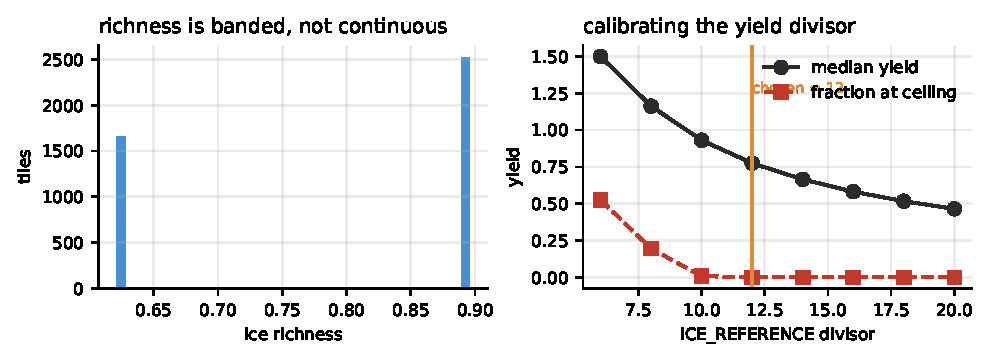
\includegraphics[width=\textwidth]{figures/ice-structure.pdf}
\caption{Left: ice richness across eight generated polar worlds, showing the
banding that follows from a quantised illumination model. Right: the yield
divisor sweep; the chosen value is the smallest at which no site saturates.}
\label{fig:ice}
\end{figure}

\section{Verification methodology}
\label{sec:verification}

\subsection{What one verification pass costs}

The model is verified by a suite of scenarios, each of which constructs a
world, drives the simulation, and asserts on the outcome. At the revision
described here the suite comprises \textbf{130 scenarios} making \textbf{594
assertions}. Executing it performs \textbf{12{,}322 simulated days} --- about
34 simulated years --- and generates \textbf{265 independent worlds}, each a
$128\times128$ field with a full solar raycast.

These figures are counted, not estimated: \texttt{e1-model-scale.mjs} wraps the
simulation's tick and world-generation entry points and runs the real suite.
We report them because they are the honest unit of reproducibility for a model
of this kind. A statement that the model "passes its tests" means little; a
statement that it survives twelve thousand simulated days across two hundred
and sixty-five independently generated worlds is a claim a reader can weigh.

\subsection{Scenarios as executable claims}

Each scenario carries a machine-readable statement of \emph{why} it exists
alongside its assertions. This is not documentation but a design constraint: a
scenario whose rationale cannot be written down is usually asserting an
implementation detail rather than a property of the model, and several were
deleted on those grounds during development.

\subsection{On counting simulation runs}

A reader may reasonably ask how many times the simulation was run in the course
of building the model. We can answer that in three parts, and only two of them
honestly.

\begin{enumerate}
\item \textbf{The cost of one pass} is exact and reproducible, and is given
  above.
\item \textbf{Runs from the point of instrumentation onward} are recorded.
  Every experiment appends to \texttt{results/ledger.json} a record of what it
  executed --- simulated days, worlds generated, and the source revision --- so
  the cost of reproducing any figure in this paper is itself a committed
  artefact.
\item \textbf{Runs before instrumentation are not recoverable.} The model was
  developed over roughly six weeks and 31 commits touching its directory,
  during which the suite was executed many times, but no count was kept and we
  decline to estimate one. Reconstructing it from commit timestamps would
  produce a number with the shape of evidence and none of the substance.
\end{enumerate}

We state this plainly because provenance is exactly the kind of claim that
invites a plausible fabrication, and because the fix --- instrument first --- is
cheap and was applied here only in retrospect. The ledger closes the gap
prospectively, not retrospectively.

\section{Results}
\label{sec:results}

\subsection{Subsurface habitation is a polar privilege}

Generating eight worlds at each of three site classes, at latitudes that would
actually produce them and with the solar geometry the model derives from that
latitude, gives the availability in Table~\ref{tab:sites}.

\begin{table}[htbp]
\centering
\caption{Habitat availability by site class. Medians over eight seeds.
Buildable surface is essentially unconstrained everywhere; subsurface
habitation is not.}
\label{tab:sites}
\begin{tabular}{lrrrrrr}
\toprule
site class & latitude & sun slope & buildable & ice tiles & bore sites & tube tiles \\
\midrule
polar    & $-85^\circ$ & 0.201 & 16{,}166 & 527 & 44 & 60 \\
highland & $-50^\circ$ & 0.489 & 16{,}135 & 383 &  2 &  0 \\
mare     & $-5^\circ$  & 0.859 & 16{,}297 &   2 &  0 &  0 \\
\bottomrule
\end{tabular}
\end{table}

The result is stark, and it was not designed in: it falls out of the
illumination coupling. At an equatorial mare site the shadow budget is so small
that the model places a median of two ice tiles on the entire map, no site
qualifies for a bore, and no rille --- and therefore no tube --- is generated at
all. Such a colony has exactly one way to house anyone: build on the surface.

The highland case is subtler and more interesting. Highland sites carry
substantial ice (383 tiles) but a median of only \emph{two} legal bore sites,
because that ice lies on slopes and a bore needs a level pad. Resource
abundance and resource \emph{accessibility} come apart, which is the sort of
distinction a whole-settlement model surfaces and a component model does not.

\begin{figure}[htbp]
\centering
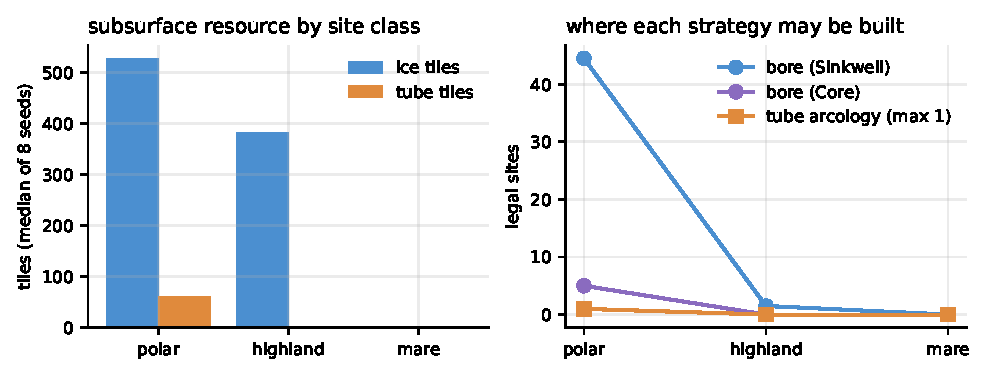
\includegraphics[width=\textwidth]{figures/site-availability.pdf}
\caption{Subsurface resource and legal sites by class. Ice is present at
highland sites but largely unusable; tubes exist only at polar sites.}
\label{fig:sites}
\end{figure}

\subsection{Arcologies buy land, not money}

Costing the three strategies on a common basis (Table~\ref{tab:econ},
Figure~\ref{fig:econ}) gives the paper's central result, and it inverts the
intuition that drove the model's design.

\begin{table}[htbp]
\centering
\caption{Habitat economics. Surface figures are for one high-density
habitation tile at its final stage. Tube figures are the median over eight
generated polar worlds; its range is $861$ to $2{,}520$ residents depending on
the tube the map produced.}
\label{tab:econ}
\begin{tabular}{lrrrr}
\toprule
strategy & residents & credits/resident & residents/kW & residents/surface tile \\
\midrule
surface tile      &    62 &   \textbf{2.4} & 31.0 &     62 \\
Sinkwell (bored)  & 1{,}100 &  58.2 & 32.4 &    122 \\
Cistern (bored)   &   480 & 170.8 & 12.0 &     53 \\
Foundry (bored)   &   405 & 182.7 &  7.8 &     45 \\
Core (bored)      & 2{,}450 & 100.0 & 25.5 &     98 \\
Tube arcology     & 2{,}295 &  41.8 & \textbf{52.2} & \textbf{2{,}295} \\
\bottomrule
\end{tabular}
\end{table}

Surface construction is between 17 and 76 times cheaper per resident than any
arcology. Whatever the case for going underground is in this model, it is not
capital efficiency.

What arcologies buy is \emph{surface area}. A tube arcology houses 2{,}295
residents while occupying a single surface tile, against 62 for the best the
surface can do --- a factor of 37. Bored arcologies achieve 45 to 122 residents
per occupied tile once their required pads are counted against them. Since the
binding constraint on a surface settlement is the ground within reach of three
utility networks, this is the currency that matters, and it is the one in which
subsurface habitation wins decisively.

The lava tube is the best deal available on every axis --- cheapest arcology
per resident, most efficient per kilowatt, and by far the most compact --- with
two compensating constraints. You get one, and its size is set by the map: the
same structure returns 861 residents on a poor tube and 2{,}520 on a generous
one, a spread of 2.9$\times$ that no decision by the player can influence. And
it returns no atmosphere, so its residents draw on pressurisation the colony
must produce elsewhere.

\begin{figure}[htbp]
\centering
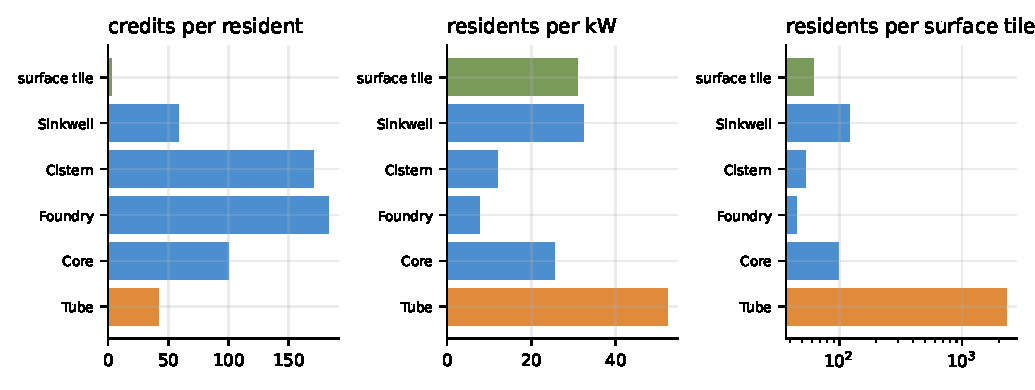
\includegraphics[width=\textwidth]{figures/habitat-economics.pdf}
\caption{The three strategies on a common basis. Surface construction wins
decisively on cost per resident; subsurface habitation wins by a larger margin
on residents per surface tile (note the logarithmic axis).}
\label{fig:econ}
\end{figure}

\section{Failure modes visible only under simulation}
\label{sec:failures}

The model includes an automated director that plays the settlement without a
human: it lays networks, zones to demand, manages a budget and builds
structures. It is useful here as an instrument, because it exercises the model
in ways a scripted test does not --- and because its failures were failures of
the \emph{model's} reasoning, not of its code.

Four such failures were found by running complete settlement histories. All
four passed every placement test throughout, because placement was never what
was broken.

\subsection{Building what cannot be used}

The director initially treated a bore like any other terrain-gated structure:
site it wherever the terrain qualifies, the moment it is affordable. But
qualifying ground for a bore is, by construction, permanently shadowed crater
floor --- precisely the ground the settlement has no other reason to expand
toward. The director bought structures that its utility networks never reached,
and each sat at one level indefinitely: a completed purchase from the outside,
and worth nothing.

Over 900 simulated days on three seeds, the naive director built twelve
subsurface structures of which \textbf{one} ever grew (Figure~\ref{fig:dir}).

\subsection{Refusing is not the same as solving}

Requiring the utilities to reach a site before building eliminated the waste
entirely --- no stalled structures on any seed --- but at a cost: the director
now built only eight structures, because it would not go to the ice at all. The
lattice grows toward valuable ground, and shadowed floors are the least
valuable ground in the model, so it never arrived.

Only when the director was given an explicit reason to walk a corridor out to
the resource did both problems resolve: fourteen structures, all growing, none
stalled. The general lesson is that a resource which is valuable only
\emph{after} you have reached it will not be reached by an agent that expands
by local value alone. That is a statement about settlement dynamics, not about
this implementation.

\begin{figure}[htbp]
\centering
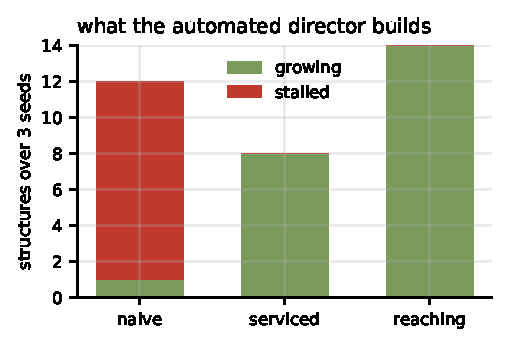
\includegraphics[width=0.5\textwidth]{figures/director-ab.pdf}
\caption{Subsurface structures built by three revisions of the automated
director over 900 simulated days on each of three seeds. The naive director
builds the most that never work.}
\label{fig:dir}
\end{figure}

\subsection{An adjacency predicate used for the wrong question}

The model asks "is this ground served by the power network?" using a predicate
that counts adjacency --- correct for deciding whether a tile may develop. The
corridor-building routine reused it to choose where to connect \emph{from},
which is a different question. A transit tube adjacent to a conduit reports
itself served and conducts nothing, so corridors anchored on one dead-ended a
single tile short, delivering transit and atmosphere to a structure with no
power.

The failure is instructive because every tile involved reported itself
correctly. Nothing was broken; a predicate was asked a question it does not
answer.

\subsection{A corridor that blocked its own successor}

Corridors laid a transit tube alongside the route for legibility. Excluding the
current route from that placement prevented a corridor from blocking itself,
but not from blocking a \emph{later} one: on one seed a site became ringed by
tubes left by its own abandoned attempts, could never be powered, and the
director re-laid the same two-tile corridor to it every 120 simulated days for
the remainder of the run.

This one is worth reporting for a methodological reason. On most of the seeds
swept during development the same defective revision built its full complement
of structures and looked entirely healthy; the fault appeared only on maps
where a corridor had to cross ground already occupied by an earlier attempt.
That is an argument for sweeping seeds rather than fixing one, and for
reporting a spread rather than a best case.

We flag explicitly that this observation, unlike the comparison in
Figure~\ref{fig:dir}, is \emph{not} among the recorded experiments. The
defective revision existed only in a working tree and was never committed, so
\texttt{e5-director-ab.mjs} --- which extracts its baselines by commit hash ---
cannot reproduce it. We report it because the failure mode is instructive, and
we mark it as unrecorded because it would otherwise carry an authority the
other results in this section have earned and it has not.

\subsection{A complexity failure hiding behind a logic failure}

Finally, the site-selection routine called a placement predicate that itself
scans the whole map, once per candidate tile --- quadratic in the map area.
This was harmless while the director placed a structure on the first tick it
could and then stopped looking. Once it was correctly refusing unreachable
sites, it never stopped looking, and the verification suite stopped completing
at all. The fix was to order the cheap network test before the expensive
placement test, reducing candidates from $16{,}384$ tiles to a few hundred.

A logic change turned a latent complexity bug into a fatal one without either
being visible in isolation. We report it because the interaction, not either
defect, is the interesting object.

\section{Limitations}
\label{sec:limitations}

This is a model of a settlement's \emph{structure}, not a prediction of any
real one. The following limitations are material to how its results should be
read.

\paragraph{Parameters are chosen for legibility, not measured.}
Costs, capacities, growth rates and power draws were selected so that the
trade-offs between strategies are visible over a few hundred simulated days.
They are not derived from engineering estimates, and the absolute numbers in
Table~\ref{tab:econ} carry no physical meaning. What is meaningful is the
\emph{ordering} and the approximate ratios between strategies, since those
follow from the model's structure rather than from any single constant.

\paragraph{The physical grounding is qualitative.}
The model reproduces the qualitative structure of polar cold traps --- ice
where illumination never reaches, richer where it reaches least --- consistent
with observations of the lunar south polar region
\citep{paige2010diviner,colaprete2010water}. It does not attempt the actual
distribution, and its ice is far more abundant and more regular than any
measurement supports. Likewise, the case for subsurface habitation rests on
regolith shielding \citep{jia2010radiation,naito2020radiation} and on the
existence and stability of intact tubes
\citep{kaku2017intact,blair2017stability}, but the model represents neither
radiation dose nor structural stability at all. A tube
in this model cannot collapse, and its roof depth is recorded but unused. Any
statement here about the desirability of going underground is a statement about
\emph{land economics under the model's assumptions}, not about safety.

\paragraph{Illumination is static in time, but not in terrain.}
Solar exposure is an eight-direction average computed at generation and never
recomputed as the Sun moves; only the shading direction is animated. This is
defensible at polar latitudes, where the point is precisely that exposure
barely changes over a cycle, and progressively less defensible toward the
equator --- which is where the model's finding that mare sites cannot support
subsurface habitation is least trustworthy.

Exposure \emph{is} recomputed locally whenever the terrain changes, whether by
the player sculpting or by a meteor strike. Deposits, however, are seeded once
at generation and never re-seeded. The asymmetry is deliberate but has a
consequence worth stating: a player can manufacture shadow and cannot
manufacture ice, so excavating a crater produces ground that looks like an ice
site by every visible criterion and holds none. Whether that is the right
model of a cold trap is arguable --- ice accumulates in shadow over geological
time, not over a season --- but it is an assumption, not a derivation.

\paragraph{One tube per world.}
The model generates at most one lava tube, on one class of site, along the path
of a single rille. Real tube systems are networks. The strong result in
Section~\ref{sec:results} that tubes are polar-only is therefore a property of
this generator, not an inference about the Moon; what the model supports is the
narrower claim that a habitat strategy whose ceiling is set by geology behaves
differently from one whose ceiling is set by budget.

\paragraph{Provenance before instrumentation is lost.}
As set out in Section~\ref{sec:verification}, the number of simulation runs
performed during development was not recorded until late, and we decline to
reconstruct it.

\paragraph{The agent is one agent.}
The director results in Section~\ref{sec:failures} describe the behaviour of a
single heuristic policy. They are evidence about what that policy does, and
only suggestive about settlement dynamics in general.

\section{Availability, reproducibility and FAIR compliance}
\label{sec:fair}

\subsection{Software}

The complete model, the verification suite, the experiments behind every figure
and table in this paper, and the source of the paper itself are in one
repository under the MIT licence:
\url{https://github.com/dr-richard-barker/LunarSims}. The model has no build
step and no runtime dependencies; it is static HTML, CSS and JavaScript, and
runs by opening a file.

\subsection{Regenerating the results}

Every number quoted in this paper is produced by a script in
\texttt{paper/experiments/}, which writes a JSON record to
\texttt{paper/results/} and appends to a run ledger. Figures are generated from
those JSON records alone --- never from the model directly --- so a figure
cannot silently disagree with the value quoted beside it. The whole chain
rebuilds with:

\begin{quote}\ttfamily
make -C paper
\end{quote}

which runs the experiments, regenerates the figures, and typesets this
document. Results are committed, so the paper builds without re-running
anything; deleting \texttt{paper/results/} forces a full regeneration.

Experiments that compare revisions of the model extract their baselines from
version control by commit hash rather than from working copies, so an A/B
comparison is reproducible from the repository alone.

\subsection{FAIR assessment}

\begin{description}
\item[Findable] The repository carries \texttt{CITATION.cff},
  \texttt{codemeta.json} and \texttt{.zenodo.json} at its root, in the
  locations GitHub and Zenodo read. A DOI is minted on deposit.
\item[Accessible] Public repository, MIT licence, no credentials, no
  dependencies, no build step. The archived snapshot is self-contained.
\item[Interoperable] Results are plain JSON with documented fields; the model
  is standard JavaScript; the manuscript is \LaTeX{} with a BibTeX
  bibliography. Nothing requires a proprietary format or tool.
\item[Reusable] The licence permits reuse and modification. Provenance is
  recorded per experiment (source revision and simulation cost). The
  limitations in Section~\ref{sec:limitations} state what the model does and
  does not support, which is a precondition for reuse that is not misuse.
\end{description}

\subsection{Fields requiring completion before deposit}

The following metadata cannot be derived from the repository and are left as
explicit placeholders rather than filled with plausible values.
\texttt{PREDEPOSIT.md} lists them with the exact file and field to edit:
author ORCID; author affiliation; the release version and tag to archive; and
the DOI, which Zenodo assigns on deposit.


\bibliographystyle{plainnat}
\bibliography{refs}

\end{document}
